\chapter{Interface}
\label{chapter:interface}

This chapter describes the interface used by the observatory staff to interact with the {\projectname} control system.

\section{Access}

The address of the {\projectname} web site is:
\begin{quotation}
\url{\projectinterfaceurl}
\end{quotation}

The web site contains the interface and documentation.

The interface is protected by passwords. The \verb|operator15| and \verb|operator21| accounts are configured with the same passwords as the RATIR interface. If in doubt, ask on the Skype chat.

The interface is only directly available to computers on the mountain-top network, although ssh port-forwarding can make it indirectly available elsewhere.

\section{Main Page}

\begin{figure}
\begin{center}
\resizebox{\linewidth}{!}{\begin{labeled}{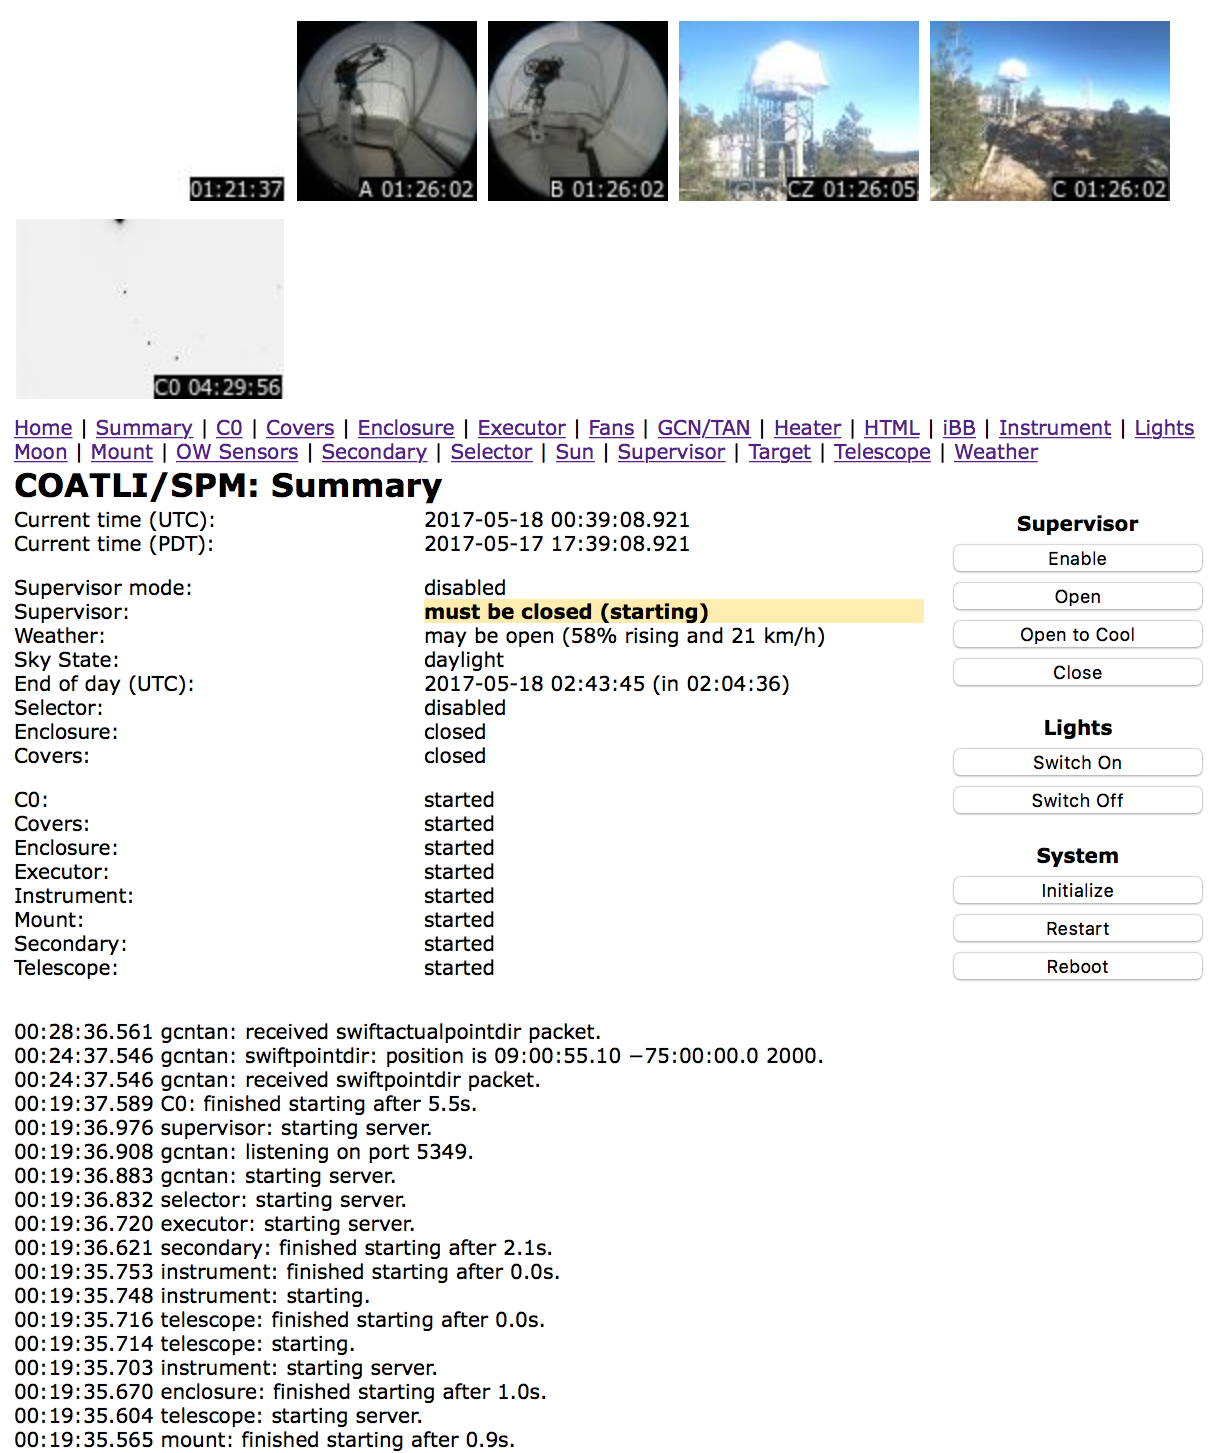
\includegraphics[width=0.8\linewidth]{figures/interface-main-page}}
\arrowandlabel{(-3.6,5.7)}{(-3.6,7)}{south}{All-Sky}
\arrowandlabel{(-1.8,5.7)}{(1,7)}{south}{Webcams}
\arrowonly{(-0.4,5.7)}{(1,7)}
\arrowonly{(+1.0,5.7)}{(1,7)}
\arrowonly{(+3.2,5.7)}{(1,7)}
\arrowandlabel{(-4.8,3.2)}{(-6,3.2)}{east}{C0}
\arrowandlabel{(-4.8,2.2)}{(-6,2.2)}{east}{Navigation}
\arrowandlabel{(-4.8,0.5)}{(-6,0.5)}{east}{Status}
\arrowandlabel{(-4.8,-1.2)}{(-6,-1.2)}{east}{Activity}
\arrowandlabel{(-4.8,-4)}{(-6,-4)}{east}{Log}
\arrowandlabel{(4.8,0.5)}{(6,0.5)}{west}{Buttons}
\end{labeled}}
\end{center}
\caption{An example of the main page of the interface. The major elements are labelled and described in the text.}
\label{figure:interface-main-page}
\end{figure}

\ifcoatlioan

\begin{figure}
\begin{center}
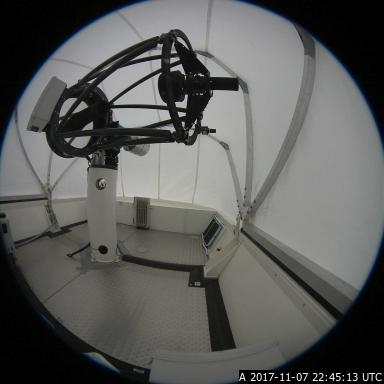
\includegraphics[width=0.8\linewidth]{figures/interface-coatlioan-webcam-a.jpg}
\end{center}
\caption{An example view from webcam A (in N corner of the enclosure looking to the SW).}
\label{figure:interface-webcam-a}
\end{figure}

\begin{figure}
\begin{center}
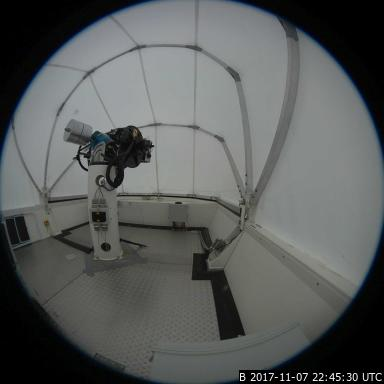
\includegraphics[width=0.8\linewidth]{figures/interface-coatlioan-webcam-b.jpg}
\end{center}
\caption{An example view from webcam B (in S corner of the enclosure looking to the NE).}
\label{figure:interface-webcam-b}
\end{figure}

\begin{figure}
\begin{center}
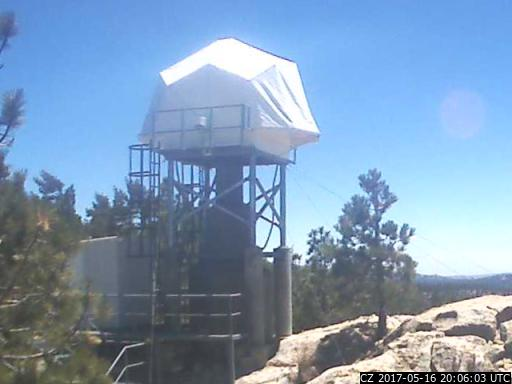
\includegraphics[width=0.8\linewidth]{figures/interface-coatlioan-webcam-cz.jpg}
\end{center}
\caption{An example view from webcam CZ (on the 84-cm telescope building looking towards {\projectname}). Webcam CZ is actually just a fixed zoom of webcam C.}
\label{figure:interface-webcam-cz}
\end{figure}

\begin{figure}
\begin{center}
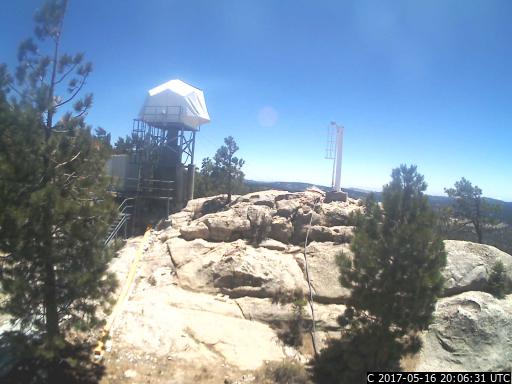
\includegraphics[width=0.8\linewidth]{figures/interface-coatlioan-webcam-c.jpg}
\end{center}
\caption{An example view from webcam C (on the 84-cm telescope building looking towards {\projectname}).}
\label{figure:interface-webcam-c}
\end{figure}

\fi

\ifddotioan

\begin{figure}
\begin{center}
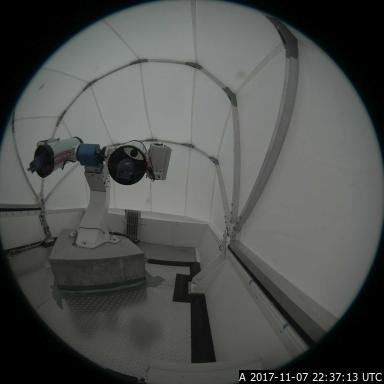
\includegraphics[width=0.8\linewidth]{figures/interface-ddotioan-webcam-a.jpg}
\end{center}
\caption{An example view from webcam A (in N corner of the enclosure looking to the SSW).}
\label{figure:interface-webcam-a}
\end{figure}

\begin{figure}
\begin{center}
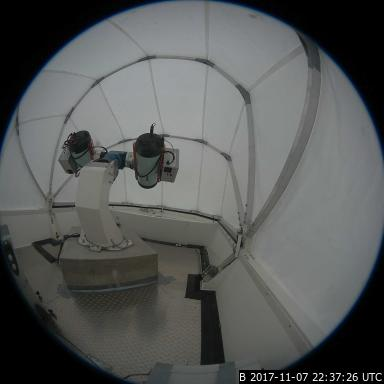
\includegraphics[width=0.8\linewidth]{figures/interface-ddotioan-webcam-b.jpg}
\end{center}
\caption{An example view from webcam B (in S corner of the enclosure looking to the NNE).}
\label{figure:interface-webcam-b}
\end{figure}

\begin{figure}
\begin{center}
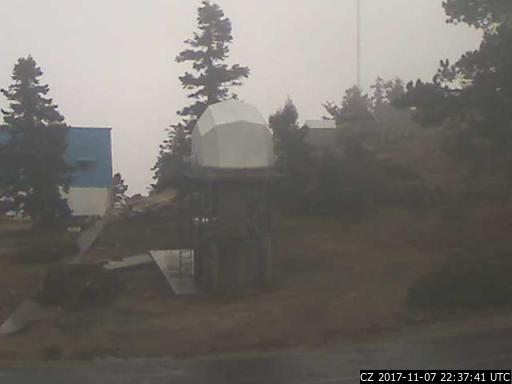
\includegraphics[width=0.8\linewidth]{figures/interface-ddotioan-webcam-cz.jpg}
\end{center}
\caption{An example view from webcam CZ (on the 84-cm telescope building looking towards {\projectname}). Webcam CZ is actually just a fixed zoom of webcam C.}
\label{figure:interface-webcam-cz}
\end{figure}

\begin{figure}
\begin{center}
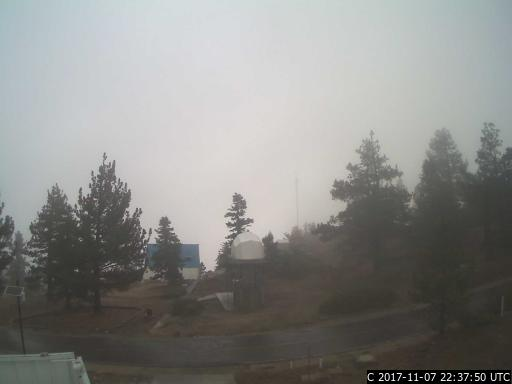
\includegraphics[width=0.8\linewidth]{figures/interface-ddotioan-webcam-c.jpg}
\end{center}
\caption{An example view from webcam C (on the 84-cm telescope building looking towards {\projectname}).}
\label{figure:interface-webcam-c}
\end{figure}

\fi

Figure~\ref{figure:interface-main-page} shows an example of the main page of the interface. The major elements of the interface are:

\begin{itemize}
\item
Thumbnail images from the webcams. Clicking on the thumbnail images brings up larger images, examples of which are shown in Figures~\ref{figure:interface-webcam-a}, \ref{figure:interface-webcam-b}, \ref{figure:interface-webcam-cz}, and \ref{figure:interface-webcam-c}. These images are useful for checking the status of the enclosure and telescope. At night, one needs to switch on the enclosure lights (see \S\ref{interface-switch-on-button}) to see anything in the webcams.  
\item
A thumbnail image from the all-sky camera. Clicking on the thumbnail image brings up a larger image. This is useful for checking for clouds.
\item
A thumbnail image of the latest image taken by the C0 detector. Clicking on the thumbnail image brings up a larger image. This is useful for checking focus.
\item
A navigation section. Clicking on these links will bring up the detailed page for the corresponding control system server. These pages are typically used by the team members to diagnose problems.
\item
A status section. In the main page this gives:
\begin{itemize}
\item
The UTC time.
\item
The civil time at the observatory (PST or PDT).
\item
The supervisor mode (“enabled”, “disabled”, “open”, “opentocool”, or “closed”).
\item
A description of whether the supervisor mode permits the enclosure to be open and why.
\item
A description of whether the current weather conditions permit the enclosure to be open and why (wind, rain, and humidity).
\item
A description of the current sky state (daylight, twilight, and night).
\item
The selector mode (enabled or disabled).
\item
The enclosure state (open or closed).
\item
The covers state (open or closed)
\end{itemize}
\item
The activity section. If a control system server activity is not “idle” (for example, if it is “started”, “initializing”, “moving”, “tracking”, “opening”, or “closing”), this is shown here. If a server activity is “idle”, it is not shown here. Thus, if all of the servers are “idle”, this section is empty.

Errors and warnings are shown here in red and yellow respectively.
\item
The log section. This section shows the latest log messages from the control system in reverse order.
\item
The buttons. These are used to interact with the control system.
\begin{itemize}
\item
Enable. Enabled the supervisor. This permits the supervisor to open and close according to the weather and sky state. Note that the supervisor only takes decisions to open, open to cool, or close if it is enabled. 
\item
Open. Force the supervisor to open and to stay open until explicitly instructed otherwise.
\item
Open to Cool. Force the supervisor to open to cool and to stay open to cool until explicitly instructed otherwise. Opening to cool opens the enclosure partially, opens the covers, and starts to cool the CCD. It is typically used at the end of the day to cool the enclosure, telescope, and CCD ready for observations after sunset.
\item
Close. Force the supervisor to open to close and to stay closed until explicitly instructed otherwise.
\label{interface-close-button}
\item
Switch On. Switch on the enclosure lights. This is useful when you want to use the webcams to check the status of the telescope or enclosure. Of course, one does not want to turn the lights on if the telescope is observing.
\label{interface-switch-on-button}
\item
Switch Off. Switch off the enclosure lights. 
\label{interface-switch-off-button}
\item
Initialize. Initialize the control system servers. Successfully initializing the servers places their hardware in a safe, closed state ready for further actions. This can be used to recover from software problems.
\label{interface-initialize-button}
\item
Restart. Schedule a restart of the control system servers for the top of the next minute. This can be used to recover from software problems.
\label{interface-restart-button}
\item
Reboot. Schedule a reboot of the control system computers for the top of the next minute. This is used to recover 
\end{itemize}
\end{itemize}

\section{Running the Interface on the Access Mac in the Shed}
\label{section:interface-access-mac}.

The interface can be run locally on the Access Mac in the Shed.

If you need to log into the Mac, use the “{\projectaccount}” account with password “{\projectaccount}”.

If the interface and Skype are not running, you can select “Open Interface” or “Open Skype” from the script menu in the upper right, as shown in Figure~\ref{figure:interface-scripts-menu}.

\begin{figure}
\begin{center}
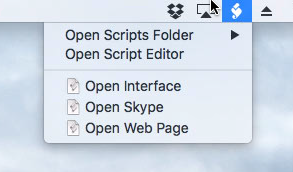
\includegraphics[width=0.4\linewidth]{figures/interface-scripts-menu.png}
\end{center}
\caption{The script menu, in the upper right, can open the interface and Skype on the Access Mac.}
\label{figure:interface-scripts-menu}
\end{figure}
